\documentclass{standalone}
\usepackage[dvipsnames]{xcolor}
\usepackage{tikz-network}

\definecolor{S}{HTML}{0b6884}
\definecolor{E}{HTML}{50b99a}
\definecolor{Ia}{HTML}{ff5e5b}
\definecolor{Is}{HTML}{ffc847}
\definecolor{R}{HTML}{7b678e}
\definecolor{D}{HTML}{bc4b51}

\definecolor{vuln}{HTML}{80475E}


\begin{document}
  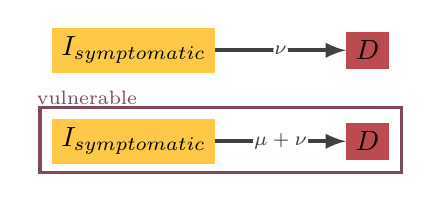
\begin{tikzpicture}[scale=0.66]
    \node at (0,  0) (Is) [shape=rectangle, fill=Is] {$I_{symptomatic}$};
    \node at (4.5,  0) (D) [shape=rectangle, fill=D] {$D$};

    \node at (0,  -1.75) (Isv) [shape=rectangle, fill=Is] {$I_{symptomatic}$};
    \node at (4.5,  -1.75) (Dv) [shape=rectangle, fill=D] {$D$};

    \draw[very thick, color=vuln] (-1.8,-1.1) rectangle (5.15,-2.35);
    \node at (-2.05,-1.24) [above right, color=vuln]{\scriptsize vulnerable};

    \Edge[Direct, label=$\nu$](Is.east)(D.west)
    \Edge[Direct, label=$\mu + \nu$](Isv.east)(Dv.west)
  \end{tikzpicture}
\end{document}
